\chapter{Penetrator}

* What kind of ice can we expect? Mud, silt etc?

\section{Drilling Methods}

\autsubsection{Mechanical Drilling}{Morten Lykke Hilligsøe}
On earth, drilling is by far the most common way of penetrating ice and has proved a viable way for recovering ice core samples at depths of up to 3.768km, reaching the underground lake Vostock, much like the mission at hand. Drilling has previously reached depths of 12.262km, and because of e.g. the oil drilling industry, experience and components are readily available. It is therefore obvious to look at the possibility of drilling through the ice on Europa.

To compare with other ice penetration methods, the following key parameters are evaluated:
\begin{itemize}
    \item Energy
	\item Time
	\item Weight
\end{itemize}
The energy required for a drill solution consists of two parts: the cutting energy and the potential energy required to move the ice. To calculate these energies, the following assumptions have been made:
\begin{itemize}
	\item Probe length:   $2m$
	\item Probe diameter:   $30cm$
	\item Europa surface gravity:   $1,3m/s^2$
	\item Europa ice density:   $124kg/m^3$
	\item Specific ice cutting energy:   $16MJ/m^3$
\end{itemize}
For cutting energy, the key parameter is the specific cutting energy. This parameter is assumed to be $16MJ/m^3$, as measured by \footnote{Greenland Ice Core: Geophysics, Geochemistry, and the Environment, Volume 33,  Chester C. Langway, Hans Oeschger, W. Dansgaard}. Other sources, e.g. \footnote{Life in Extreme Environments, Ricardo Amils, J. Cynan Ellis-Evans, Helmut Hinghofer-Szalkay}, have measured specific cutting energies of similar size, at $20MJ/m^3$.

The result is a cutting energy of:
\begin{equation}
    E_{Cut} = A \cdot E_{Specific}
\end{equation}
\begin{equation}
    E_{Cut} = (0.15m)^2 \cdot \pi \cdot 16MJ/m^3 \cdot 1000m/km = 1.130 MJ/km
\end{equation}
The potential energy required to move the ice, will have to at least match the volume of ice which the penetrator probe displaces.  The result is a minimum potential energy of:
\begin{multline}
E_{pot} = m \cdot g \cdot h = \rho \cdot V \cdot g \cdot h\\
 = (0.15m)^2 \cdot \pi \cdot 124kg/m^3 \cdot 1.3m/s^2 \cdot 2m \cdot 1000m/km = 22.8 kJ/km
\end{multline}
Where the surface gravity of Europa is provided by \footnote{\url{https://en.wikipedia.org/wiki/Europa_(moon)}}, and the ice density $\rho$ is calculated from the value on earth at -180°C as stated in \footnote{\url{https://en.wikipedia.org/wiki/Properties_of_water}}:
\begin{equation}
\rho_{Europa} = \rho_{Earth} \cdot \frac{g_{Europa}}{g_{Earth}}
\end{equation}
\begin{equation}
\rho_{Europa} = 934kg/m^3 \cdot \frac{9.82m/s^2}{1.3m/s^2} = 124kg/m^3
\end{equation}
Compared to the cutting energy, the potential energy seems insignificant. However, this might not be a realistic assumption, since the shaved ice will most likely take up more space than the equivalent amount of solid ice, and will therefore have to either be moved additionally, or compressed. Also, the drilling equipment will most likely take up a much greater volume than the probe itself, and this energy must therefore be expected to increase in multifold.

But even if the energy required to drill through the ice is reasonable, drilling time and system weight are key parameters. Table \ref{tab:ice_core_drilling}\footnote{A Fast Mechanical-Access Drill for Polar Glaciology, Paleoclimatology, Geology, Tectonics, and Biology, Gary D. Clow and Bruce Koci}  presents these key parameter for two currently employed methods of ice drilling: Ice Core Drilling (ICD) and Hot-Water Drilling (HWD), as well as a solution based on Coiled Tubing Drillling for Ice (CTDI), which have yet to be employed in ice drilling projects. As seen from this table, drilling a 3.5km borehole can take as little as 6-8 days by using a CTDI system. However, the weights of such systems are in the tens-hundreds of tonnes, making ice drilling systems impossible to bring as payload on a rocket.

\begin{figure}[htb]
  \centering
  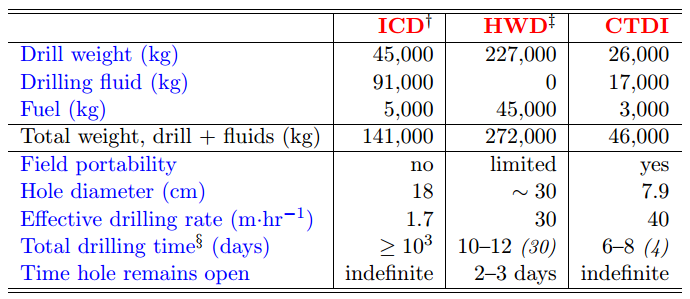
\includegraphics[width=0.7\textwidth]{figures/mlh/table_ice_core_drilling}
  \caption{Comparison of the weights and times required to drill a 3.5-km borehole through ice using ice-coring, hot-water, and CTDI drilling systems.}
  \label{tab:ice_core_drilling}
\end{figure}

Figures \ref{fig:ICD}, \ref{fig:HWD} and \ref{fig:CTDI} illustrates the three methods presented in table \ref{tab:ice_core_drilling}.

\begin{figure}[htb]
  \centering
  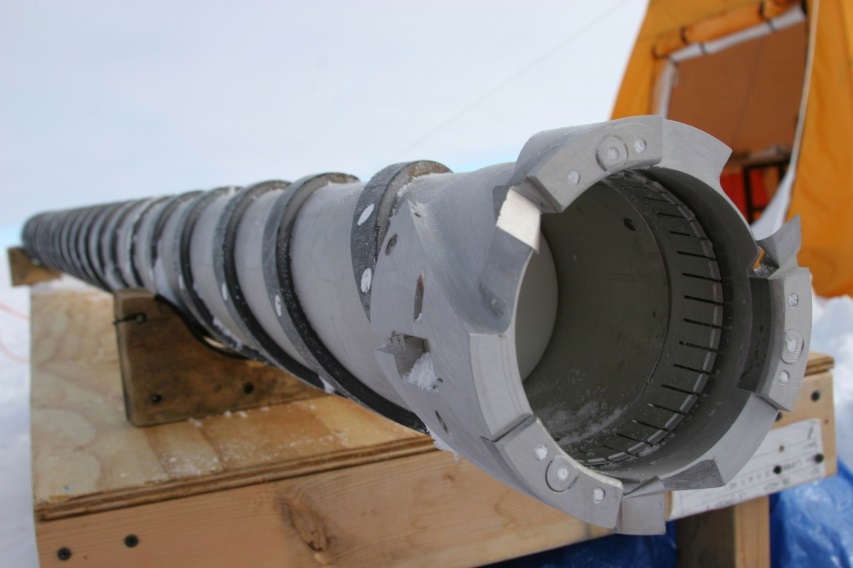
\includegraphics[width=0.5\textwidth]{figures/mlh/ICD}
  \caption{The hollow drill of an Ice Core Drilling, which enables researchers to retrieve pure ice core samples.}
  \label{fig:ICD}
\end{figure}
\begin{figure}[htb]
  \centering
  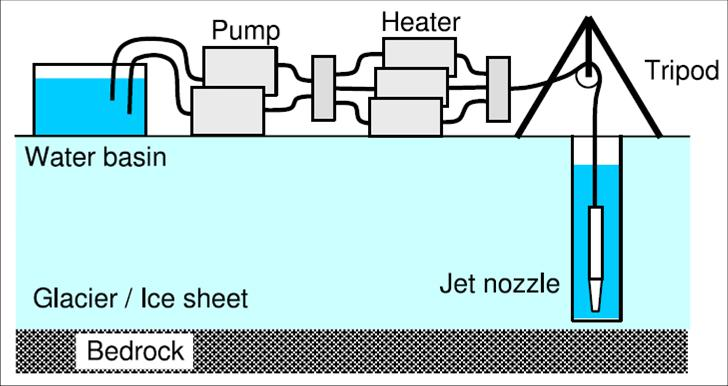
\includegraphics[width=0.5\textwidth]{figures/mlh/HWD}
  \caption{Principles of Hot Water Drilling in ice.}
  \label{fig:HWD}
\end{figure}
\begin{figure}[htb]
  \centering
  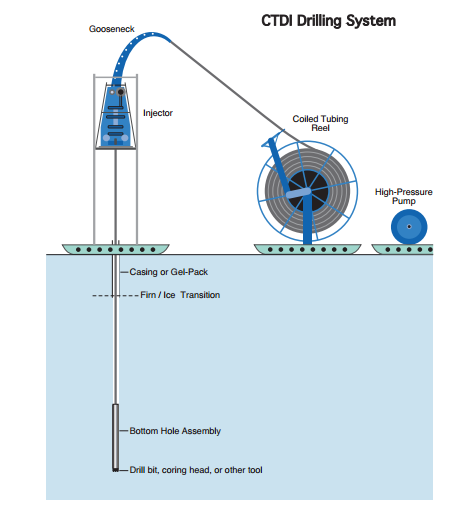
\includegraphics[width=0.6\textwidth]{figures/mlh/CTDI}
  \caption{Principles of Coiled Tube Drilling in Ice.}
  \label{fig:CTDI}
\end{figure}

\subsection{Chemical Drilling}

\subsection{Explosive Drilling}

\subsection{Sputtering}

\autsubsection{Laser Drilling}{Bhaaeddin Alhomsi and Paul Connetable}

Lasers may provide another methodto dig through the layer of ice. High-power lasers exceeding 10 kW have been developed and widely used for industry (Gapontsev et al., 2009; Richardson et al., 2010; Fujita et al., 2010). For example, a recent laboratory test using a 1.6-kW pulsed Nd:YAG 1.064 $\mu$m wavelength laser beam determined the energy required to spall, melt, and
vaporize several rock samples for oil and gas well drilling. The required energy (specific energy) depends on the absorption properties of each rock sample as well as the reflective properties of the rock surface  (Gahan and Parker, 2001; Xu et al., 2003). A new laser-mechanical bit for laser spallation of rock to give an optimum drilling mechanism
was found to reduce rig time and increase drilling efficiency (Pooniwala, 2006).More recently, a 20-kWlaserwas delivered through a 1500 m-long optical fiber cable and shown to be able to efficiently drill oil and gas wells (Hecht, 2012). Finally, in the project VALKYRIE,
ice was drilled by a self-contained "intelligent ice penetrator", a 5 kW laser at 1070 nm wavelength (Siegel et al., 2013)(Stone et al., 2014).
Test of VALKYRIE between 2010 and 2013 used high-power optical energy transfer over km-scale distances and tested the feasibility of a vehicle deployed optical waveguide. Thus, a laser-drill system may be useful for ice-sheet applications, including the search for life in extreme environmental conditions here on Earth as well as outer planets.
With continual improvements, laser drilling may develop advantages over other methods for ice.We investigate here the behaviour of laser melting of ice and snow with an infrared laser for the potential use as a drill.

\subsubsection{Characteristics of light absorbance in ice}

The first step before selecting a laser is to analyze the spectral absorption of the medium we want to dig through. Therefore, the ice transmittance spectrum is displayed in Figure \ref{IceAbsorbance}. One can observe on this figure peaks of absorption, at around $10^{-5}~m$, and around $6\times10^{-5}~m$. The best suited lasers for digging through ice would have to emit at these frequencies.

Hence, we use a $CO_2$ laser, which is a relatively inexpensive common infrared gas laser (Patel, 1964) with fundamental lines from 9.2 to 10.8 $\mu$m and used in both pulse and continuous wave (CW) mode. For ice, an earlier study demonstrated the potential of $CO_2$ laser irradiation to help breakup nautical sea-ice (Clark et al.,  1973), but the laser has apparently not previously been used for snow and ice drilling.

\begin{figure}[htb]
\centering
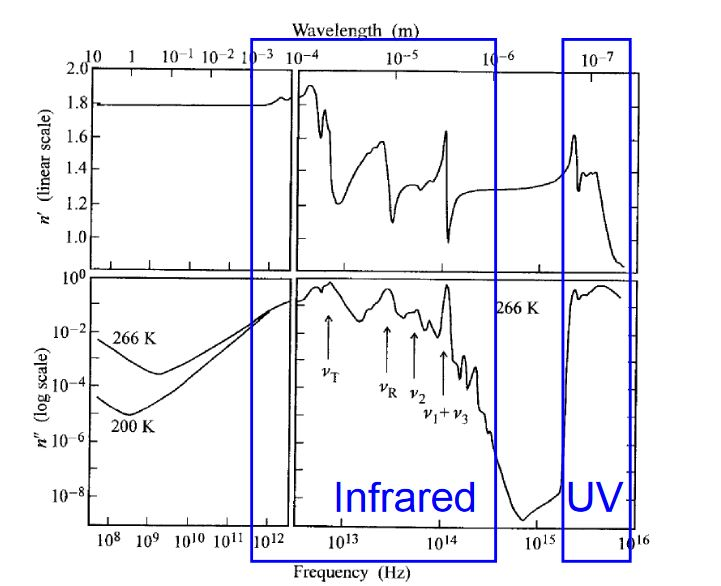
\includegraphics[width=.48\textwidth]{figures/laser-drilling/iceabsorbance}
\caption{Reported values of transmittance in ice}
\label{IceAbsorbance}
\end{figure}

The absorption of light in ice depends on the complex refractive index of ice. According to data in a previous study (Warren and Brandt, 2008), the absorption coefficient of ice significantly increases from the near- to mid-infra-red region, reaching a value of about $\unit[628.3]{cm^{-1}}$ at the $CO_2$ laser wavelength of 10.6 $\mu$m. Ice absorbs almost 100\% of the light intensity at 10.6 and 1.064 $\mu$m within a penetration distance of 0.01 and 2 cm, as shown in Figure \ref{fig:bh1}.

\begin{figure}[htb]
\centering
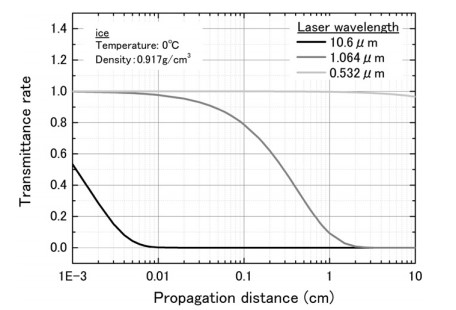
\includegraphics[width=.48\textwidth]{figures/laser-drilling/bh1.jpg}
\caption{Characteristics of light absorbance in ice}
\label{fig:bh1}
\end{figure}

\subsubsection{Melting studies of ice and snow by $CO_2$ laser}

A $CO_2$ laser can be used to melt ice. The $CO_2$ laser at 10.6 $\mu$m (25.5 W) and a beam diameter of 1.0 cm, a wavelength at which ice strongly absorbs, to drill (via melting) through ice. The resulting drilling speed is measured at several irradiation intensities, ice-snow densities, and beam angles relative to the horizontal axis.
The melting speed increases with increasing laser intensity and with decreasing ice density, as shown in Figure \ref{fig:bh2}. The melting speed ratio between ice ($\unitfrac[917]{kg}{m^3}$) and the lowest-density snow ($\unitfrac[153]{kg}{m^3}$) is 4-5, slightly less than the value of \~6 expected from the density ratio \cite{lasermelt}. The reason for this discrepancy could be explained by the snow having a greater reflectivity than solid ice. The melting speed decreases with increasing snow density.

\begin{figure}[htb]
\centering
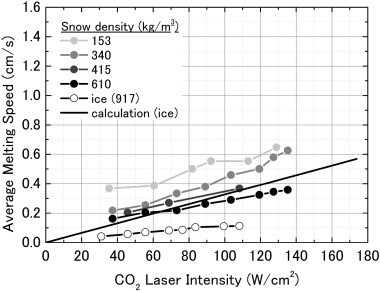
\includegraphics[width=.48\textwidth]{figures/laser-drilling/bh2.jpg}
\caption{Relation between laser intensity and melting speed}
\label{fig:bh2}
\end{figure}

\subsubsection{Results}

Unfortunately, the experimental results indicate that the melt-water accumulates in the hole and reduces the melting speed of ice and a pump system could not be installed due to a high distance.
Moreover, since the energy source brought in the penetrator is a RTG, using a laser would require to transform the thermal energy produced by the RTG in electric energy. Such a conversion has an efficiency of about 20~\%. If we add to that the fact that the best $CO_{2}$ lasers also have efficiencies up to only 20~\%, the best efficiency achievable on this drilling method is of about 4~\%with the current technology. This is still while assuming that the ice absorbs all of the energy sent by the laser, which is not the case. It means that the efficiency of such a drilling method would be extremely low, and thus not indicated for our mission.
In future studies, it will be necessary to investigate quantitatively several additional factors. These include the optical-fiber coupled laser intensities required for deep drilling, and a method to pump melted water. Despite these hurdles, laser drilling is a promising technology for ice drilling. Lasers are indeed capable of delivering very high powers precisely. Furthermore, the main reason for low $CO_{2}$ lasers' efficiency is the power consumed for cooling the body of the laser. This efficiency could then go up if a laser specifically designed for our mission was done, since it could use the cold surroundings of the penetrator to cool down.


\subsection{Light Concentration Drilling}

\subsection{Melting}


* Water transportation from tip to the end of the penetrator (ref section about convection flow)

* Should measure flow of the water - descent rate

* Water flow to the instruments. Will have to use a pump in order to increase the flow rate.

* Measure conductivity of the water.

\section{RTG design}

\autsubsection{Radioactive Sources}{Jean-Paul Breuer}
A Radioisotope Thermal Generator (RTG), is essentially an nuclear battery that uses thermocouplers to convert the heat released by a selected radioactive source into electricity. Many radioactive sources exist which could serve the purpose of fuel for the RTG specific to this mission, but not all of the known radioactive isotopes would be efficient or viable for the task. There are three important characteristics to keep in mind when attempting to select the ideal radioactive isotopes.

An important criteria is the half-life time of the selected isotope. The minimum viable time is computed based on highly conservative estimates, where the main condition is that the isotope must still be able to provide sufficient energy for the instrumentation well after the coasting phase and the melting phase. Dependent on which rocket the mission is given, the coasting time could be anywhere between 2 and 8 years, and dependent on which landing site is chosen on the surface of Europa, the melting phase could take between 1 and 10 years (at a 200 day per km of ice melting rate). 

The amount of energy per time released is inversely proportional to its half life, so the ideal radioactive candidate will require a half life in the magnitude of several decades. To sit well within the mass, power, and volume budget, another criteria is that it must produce sufficiently large amount of power per mass and volume. The last criteria is that the type of radiation is easily absorbed and converted into thermal radiation, in other words, maximize the alpha particles released, and minimize the gamma, neutron, and penetrating radiation.

Given the three main criteria, it is possible to exclude many isotopes immediately, although the most likely candidates are given in Table \ref{tab:isotopes}. Other more known and available isotopes, such as Uranium, have a long half-life time and as such do not generate enough energy per time to be able to sufficiently provide the heat required for ice melting.

\begin{table}[h!]
	\begin{tabular}{c|c|c|c|c}
		Candidate Isotopes & Half-Life & Power & Gamma, Neutron Level & Availability\\
		\hline
		Plutonium-238 & 87.7 years & $\sim$ 671 W/kg & Low & Low\\
		Strontium-90 & 28.8 years & $\sim$ 446 W/kg & Medium & High\\
		Americium-241 & 432 years & $\sim$ 135 W/kg & Low & High\\
		Polonium-210 & 138 days & $\sim$ 171269 W/kg & Low & Low\\
	\end{tabular}
	\caption{Table of radioactive sources that can be used for the RTG, half-life, power, and other information are given. \label{tab:isotopes}}
\end{table}

As can be seen from the table, Plutonium-238 and Americium-241 would seem like viable candidates for this mission; however, Americium requires further shielding due to it releasing gamma radiation along with the alpha particles.

\autsubsection{Radiation from Pu238}{Ricard Lladó Grove}
After looking at the different materials, Plutonium-238 (Pu238) is radioactive material that is going to be used for the mission due to the the half-life of 87.7 and the minimum radiation of gamma and neutrons. 

The probability of a alpha-decay from a Pu238-atom is close to 100\%: 
\begin{equation}
^{238}\text{Ph} \quad \rightarrow \quad ^{234}\text{U} \quad + \quad ^4 \text{He}
\end{equation}
The alpha particle is relatively big with two protons and two neutrons and is therefore easy to shield against. Even if the possibility of an alpha decay is close to almost certain, there is a small possibility of either a spontaneous fission or a cluster decay. A spontaneous fission happens for heavy atoms, where the atom split into two almost equal sized daughter atoms and a number of free neutrons. The possibility of a spontaneous fission for Pu238 is $1.9 \cdot 10^{-7}\%$, but with more than $10^{24}$ atoms for each kg of plutonium, it is certain to happen. The daughter atoms can vary. A cluster decay is something between an alpha decay and spontaneous decay where a cluster of protons and neutrons are emitted. For the Pu238 there is a $1.4 \cdot 10^{-14}\%$ chance that a Si32-atom is emitted leaving a Hg206-atom, and a $6 \cdot 10^{-15}\%$ chance that a Mg30-atom and a Mg28-atom is emitted leaving an Yb180-atom. The daughter isotopes are also radioactive and are most likely to emit a beta-particle. This particle is either an electron or a positron depending on the charge of the particle with a mass much smaller than neutron or proton but since it has an electric charge it can rather easily be stop by a shielding metal.\\

\noindent
A bigger problem is the free neutrons that for example are emitted due to a spontaneous fission.  The neutrons do not have any electric charge and therefore they will not be stopped by an electric field making them extremely penetrating. To stop a neutron is has to be absorbed by a nucleus or collide with a particle with same speed but opposite velocity and mass as the neutron. Since the materials used to shield alpha and beta particles, for example lead, has a rather small cross-section and hew nuclei per unit mass, hence the neutron can easily pass trough the shielding. Furthermore if the neutron is absorbed to the atom it is likely that the new atom is radioactive as well. Therefore it is important to stop the neutrons, because they can cause a lot of damage if they hit the instruments on board the penetrator. In order to do so protium, a hydrogen atom with no neutron, can be used to absorb the neutron creating in deuterium. Water has a high number density to mass ratio, and is hereby optimal to use as a shielding against the free neutrons.


\autsubsection{Shielding}{Ricard Lladó Grove}
As mentioned a typical shielding material is lead, but for this case zirconium would be a better choice, first of all because it has a melting temperature that is three times higher than lead, and second of all because the material is lighter. It is still not possible to stop the free neutrons, where we instead will use water. First the Plutonium will be surrounded by the zirconium, afterwards a layer of water and in the end some thermocouplers will generate electricity from the heat. 

\autsubsection{Heat Generation}{Ricard Lladó Grove}
To calculate how much energy one alpha decay will produce, the energy equation derived from Einstein is used:
\begin{equation}
\begin{aligned} 
\text{$E_{atom}$} & ={} mc^2 \\
& = (m_{Pu238} - [m_{U234} + m_{He4}]) \cdot c^2 \\
& = (238.049559894U - [234.040952088U + 4.00150646649U])\\
& \cdot 1.66053904020\cdot 10^{-27}\text{kg} \cdot 2.99\cdot 10^8 \text{m/s}\\
& = 1.06\cdot 10^{-12} J 
\end{aligned}
\end{equation}
When knowing how much one decay will produce of thermal energy, the number of decays in a radioactive material can be calculated as following:
\begin{equation}
A = A_0 \cdot 2^{\frac{t}{\tau}}
\end{equation}
where \textit{$A_0$} is the initial number of atoms in a lump of a radioactive material, \textit{A} is the atoms left in the material after a specific time, \textit{t}, with a half-life of  \textit{$\tau$}. The energy produced by one kg of Pu238 over a timespan of one second will then be: 
\begin{equation}
\begin{aligned} 
\text{$E_{kg}$} & ={} E_{atom} \cdot [A_0 - A] \\
& = E_{atom} \cdot \left[A_0 - A_0 \cdot 2^{\frac{t}{\tau}}\right] \\
& = E_{atom}  \cdot \left[\frac{1}{m_{Pu238}} - \frac{2^{\frac{t}{\tau}}}{m_{Pu238}} \right] \\
& = 671 J
\end{aligned}
\end{equation}
We here see that for each kg of Pu238, 671W energy is generated in form of thermal energy. Since the amount of Pu238 decreases for each decay, the generated energy will also decrease, but rather slowly since the half life is 87.7 years. 
After the decay to U234, the uranium is also radioactive, undergoing an alpha decay as well. The lifetime is more than 2400 years and therefore the decay from this isotope is much more protracted. The decay chain from Pu238 will end with the stable isotope Pb206 after 12 decays from either alpha or beta decay. \\

\noindent
Plutonium is normally not used in its pure form. Normally it is processed into the chemical plutonium dioxide, PuO2 \cite{website:plutoniumoxide}. This ceramic is more stable and in case of an accident at launch or re-entry pure plutonium would be scattered into small pieces on a large area under the accident where PuO2 would more or less stay as one big lump which would make it easy to clean up and prevent a radioactive release. Furthermore the melting temperature is $2.660^oC$ and has a low solubility in water, meaning that it does not easily dissolve in water. When using plutonium dioxide compared to pure plutonium the power produced per kg will also decrease. Pu238 weights about 238 atomic units and oxygen weights about 16 atomic units. By calculating the percentage of oxygen compared to plutonium an estimate of the power per mass can be found: 
\begin{equation}
\text{Percentage Plutonium in PuO2} = \frac{p_{Pu} - p_{O2}}{p_{Pu}}\cdot 100\% = \frac{238 - 32}{238}\cdot 100\% = 86.5\% 
\end{equation}
Hereby the heat production is reduced from 671 J to $671J \cdot 0.865 = 580 J$. \\



\noindent
Since we need 2kW of thermal energy and around 100W as electrical energy for the instruments on the penetrator we would need around 5 kg of plutonium. Some extra plutonium is needed because the amount of radioactive material decreases with time, and since the mission takes a couple of years the heat generation have decreased a factor 
\begin{equation}
N = N_t \left(\frac{1}{2}\right)^{t/\tau} 
\end{equation}

\noindent
With a density of 19816 kg$/m^3$, with a mass of 5 kg we would need a a plutonium rod that is 30 cm long and 1.65 cm in radius. It is a good idea that the plutonium has a high surface area compared to the volume, because the heat was to be distributed to the water running in the heat pipes(maybe). Furthermore it is a good thing that the plutonium has the same shape as the penetrator. (Explanation to come) 


\autsubsection{Heat pipes}{Ricard Lladó Grove}
To distribute the heat that is generated from the plutonium. In order to do so, the water will be under high pressure. If the pressure inside the pipe system is 50 bar, or around 5 MPa, the water has a boiling temperature at $264^\circ$C. This will give some advantages for the system in the sense that it is almost impossible to maintain a temperature below $100^\circ$C which is waters normal boiling point, when transporting 2kW of heat.\\

\noindent
The pipe system will consist of pipes surrounding the RTG in the bottom and middle of the penetrator. Since the RTG is 30 cm long the pipes will be this as well with 18 tubes cut in half. The water will then flow out to the 18 tubes in the outer part of the RTG. Since most of the heat of generated should be directed downwards 12 of the tubes only cover the lowest $1/4$ of the penetrator. The other 6 tubes will go all the way to the top of the penetrator in order to ensure that the penetrator will not freeze in because the top of the penetrator is too cold. With an internal pressure of 5MPa, the thickness of the tubes that have water in them will be around 1 mm depending on the material if the other radius of the tubes are 1.48 cm. The heat pipe system will then weight around 6 kg. Furthermore the system will take up 6.5 liters of space. 

Insert image of top view of the pipe system and RTG. 
Insert image of a sideways look of the system.

\autsection{Pressure Distribution Europa}{Ricard Lladó Grove} 

Secondly the gravitational acceleration is set to be $1.314 \frac{m}{s^2}$, and has been calculated by 
\begin{equation}
g = \frac{GM}{r^2}
\end{equation} 
where $G = 6.67\cdot 10^{-11}\frac{m^3}{s^2 kg}$ is the gravitational constant, $M = 4.8\cdot 10^{22}$kg is the mass of Europa and $r = 1560.8$ km is the radius of Europa.  We see that the further the penetrator melts its way down through the ice the radius decreases. The mass distribution will also change since now there will be mass above you which will pull you in that direction, but on the other hand you will be closer to the mass on the other side of the planet. Therefore the change in gravitational acceleration depends on the distribution of the mass on Europa, and especially how dense the core is which in this case is unknown. 



\section{Selected Design}

* Sketch of overall design (use 3D models for the ice melting simulations)

\subsection{Melting through the ice} % Lukas, KSL

\subsection{RTG on Top}

\subsection{RTG on Bottom}

* How do we protect the rest of the instruments against the radiation?


\subsection{Thermal Design}

\subsection{Water Convection}

\autsection{Penetrator thickness}{Ricard Lladó Grove} 
\begin{equation}\label{eq:pressure}
\sigma = \frac{-2 P_{ext}\cdot r_{outer}^2}{r_{outer}^2-r_{inner}^2}/ + \frac{P_{int}\cdot (r_{outer}^2+r_{inner}^2)}{(r_{outer}^2-r_{inner}^2)}
\end{equation}
where $\sigma$ is the stress on the material, $P_{ext}$ and $P_{int}$ is the external and internal pressure, $r_{outer}$ and $r_{inner}$ is the outer and inner radius. 


\section{Anchor Design}
\autsubsection{Buoyancy}{Ricard Lladó Grove}
One way to anchor the penetrator is trough buoyancy. In general buoyancy is an upward force that is exerted to an object by the surrounded fluid. For an object immersed in a fluid, the force acting on the object is gravity and buoyancy given by:
\begin{subequations}
\begin{equation}\label{eq:bouyancy1}
F_{gravity} = m_{object} \cdot g
\end{equation}
\begin{equation} \label{eq:bouyancy2}
F_{buoyancy} = \rho_{fluid}\cdot g \cdot V_{immersed} 
\end{equation}
\end{subequations}
where $g$ is the gravitational acceleration, $\rho$ is density, $V$ is volume of the immersed part of the object and $m$ is mass.  In our case the object is the penetrator and the fluid that the penetrator is immersed into is assumed to be pure water. In order to use buoyancy as the anchor of the penetrator, it has to cancel out the force of the gravity that will pull the penetrator downwards i.e make it sink. We can hereby equal equation \ref{eq:bouyancy1} and \ref{eq:bouyancy2}:
\begin{subequations}
\begin{equation*}\label{eq:bou1}
F_{gravity} = F_{buoyancy} \quad \rightarrow \quad m_{penetrator}\cdot g_{Europa} = \rho_{fluid}\cdot g_{Europa} \cdot V_{immersed}   \quad \rightarrow 
\end{equation*}
\begin{equation} \label{eq:bou2}
V_{immersed} = \frac{m_{penetrator}}{\rho_{fluid}}
\end{equation}
\end{subequations}
First of all we see that the gravitational acceleration of Europa cancels out in both equations, which simplifies the expression. It is desired to calculate the volume that is needed in order to the force of the buoyancy to be great enough to lift the mass of the penetrator hence cancel out the gravity. The mass of the penetrator is in our mission straw man set to be maximum 180 kg even though it is only an assumption  If the mass of the penetrator shows to actually be lower than expected a lower volume would be needed. The density of the water is set to 1000 $\frac{m^3}{kg}$ which is the density of pure water. It is not known how salty the water if it contains salt, but the density of salt water is slightly higher then water without salt, and hereby the buoyancy force would be higher and a smaller volume is needed, so by using pure water we get a conservative value of the volume. By inserting the value we end up with the volume needed to carry the penetrator in pure water:
\begin{equation}
V_{needed} = 0.180 m^3 \rightarrow 180 \text{litres}
\end{equation}
Since the penetrator is 48.2 litres the extra required volume is about 132 litres. There are many ways to use buoyancy. Submarines have a ballast tank that they can fill with either water or oil. Since oil is about 0.8 times as dense as water this will create a buoyancy and depending on how much water is displaced. This solution is not useful for this penetrator since a huge reservoir of oil is needed which would take up more space and mass than is to dispersal. Another solution is to have an inflatable reservoir that will expand when the internal pressure increases. An illustration of such a solution is showed in figure \ref{fig:bouyancy1}.
\begin{figure}[htb]
  \centering
  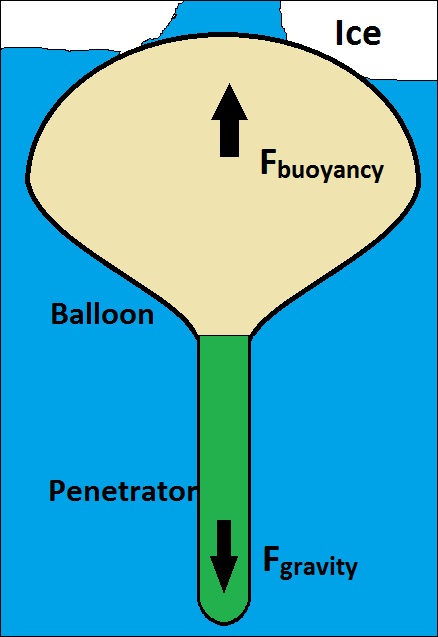
\includegraphics[width=0.5\textwidth]{figures/Ricardo/Buoyancy1.png}
  \caption{Illustration of the immersed penetrator with the inflated balloon to reach equilibrium between the buoyancy force and the gravitational force}
  \label{fig:buoyancy1}
\end{figure}
When the penetrator melts through the last ice the velocity of the penetrator will increase because the it will sink though the water. With a short delay to ensure that the penetrator is surrounded by water, a trigger should inflate a balloon attached to the penetrator. The balloon should have a volume of at least 132 litres since we would probably like a small lift of the buoyancy. The most suitable place for the balloon to be inflated is above the penetrator since the balloon will have the uplift required to cancel out the effect of gravity. Hereby this will be the most stable situation even though it will complicate the communication to the lander since the antenna should be above the balloon. This is doable but not the most desired solution. In this case a volume of 132 litres should be obtained when having the same internal and external pressure. One way to obtain this is by having a pressure vessel with a huge internal pressure. If the volume of the penetrator is 10 litres the pressure inside the vessel should be 13.2 times bigger than the external pressure which is 12MPa in 10 km depth. Hereby an internal pressure of more than 160MPa is needed in the pressure vessel. In this way when the pressure of the pressure vessel is released into the balloon it would expand 13.2 times which is 132 litres. The problem with this solution is that a pressure vessel that can withstand such a pressure has to be relatively big and hereby also heavy. As an example the equation \ref{eq:pressure} can be used to calculate the properties of such a strong pressure vessel.  if using titanium as the pressure vessel and assuming that the vessel is a sphere which is the strongest structure to withstand pressure, the radius would be 9.5 cm and the thickness had to be about 4 cm to withstand the 160MPa internal pressure, which would mean a mass of about 30 kg. This will make the buoyancy anchoring disadvantageous against other anchoring methods. \\

Another way to inflate the balloon is by having a chemical reaction that will produce a quantity of gas.


\noindent 
Even though it is disadvantageous it would be good to see if the buoyancy is even possible for these high pressures since almost all gases are liquid or even solid at these high pressures. Since a liquid is almost incompressible it can be compressed to the desired pressure without taking much space. The problem is then that when released the pressure has to be low enough for the liquid to evaporate. To give an example the gas CO2 can be selected. The Phase diagram of CO2 is illustrated in figure \ref{fig:CO2phase}
\begin{figure}[htb]
\centering
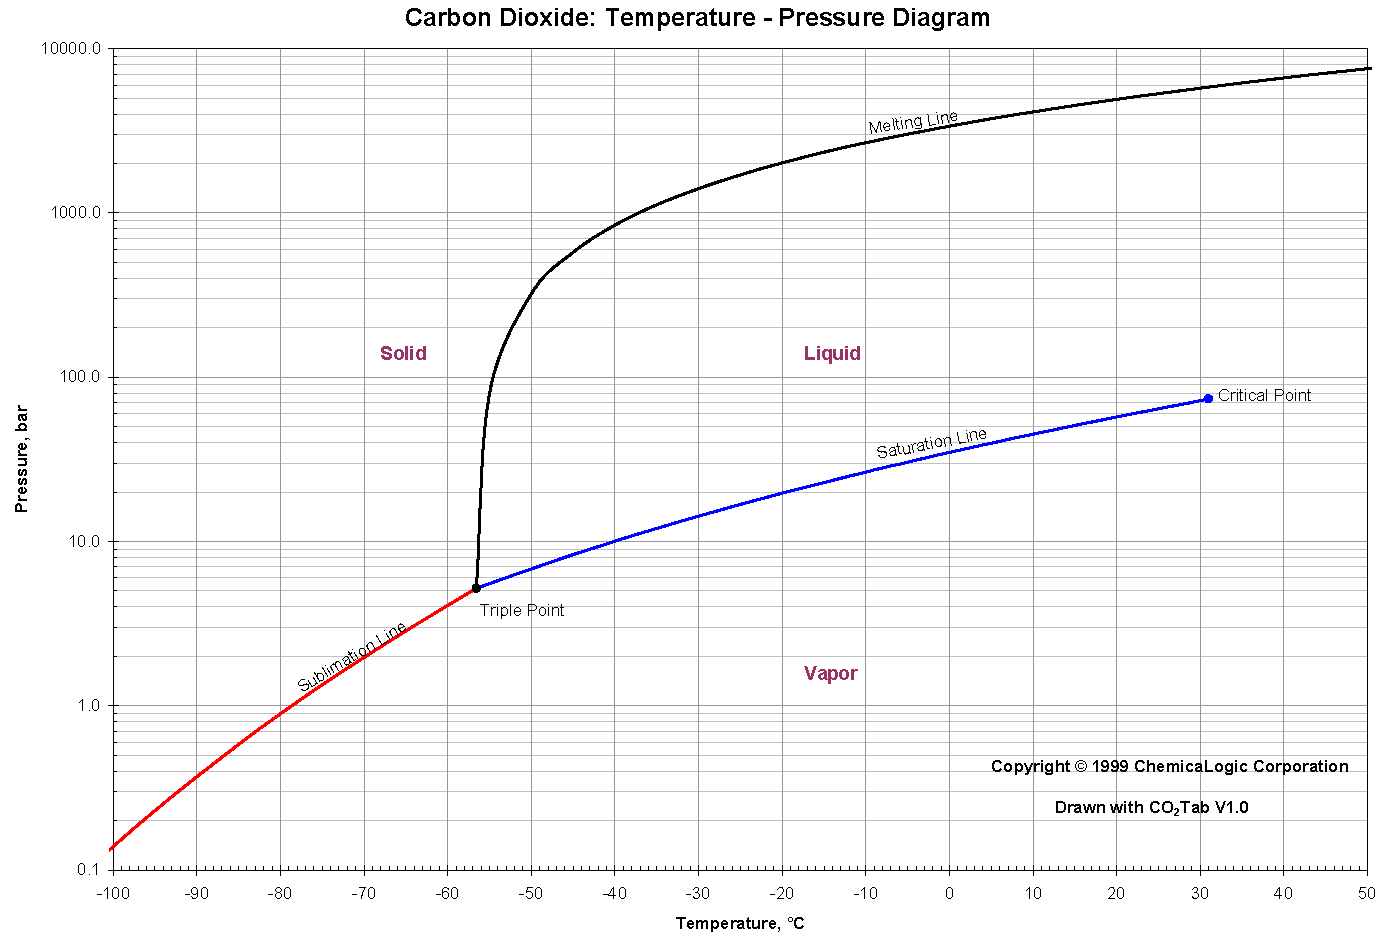
\includegraphics[width=0.9\textwidth]{figures/Ricardo/co2_phase_diagram}\caption{Phase diagram of CO2. From: \url{http://www.chemicalogic.com/Documents/co2_phase_diagram.pdf}}
\label{fig:CO2phase}
\end{figure}
With the balloon above the penetrator, it will be surrounded by water that has a temperature close to the freezing point and hereby the temperature of the gas would be almost the same as the temperature of the surrounding water which is around 273 K, corresponding to $0^oC$. In figure \ref{fig:CO2phase} the vaporization point corresponding to this temperature is 35 bar. Since we have to assume the worst case scenario the depth of the ice could be up to 10 km deep, the pressure is approximately 120 bar. This is a huge problem since CO2 at this pressure hereby would not evaporate from the liquid pressure vessel. One solution is to increase the temperature. The critical point for CO2 is about $30^oC$ where the pressure is just above 70 bar. In principle this means that CO2 cannot be  used for a depth of 10 km. This means that another gas has to be used in order to make buoyancy work at this pressure. For water the phase diagram is illustrated earlier we see that at temperatures around 600 Kelvin the vaporization point is about 120 bar. A possible solution these high temperatures would be to have the balloon surrounding the penetrator and use the heat produced by the RTG to warm up the gas. This would produce problems since the density of the gas would be less than the density of the penetrator and hereby in worst case scenario the penetrator would tilt or flip and all communication would be lost. Furthermore the heating of the gas would last for relatively long time and hereby the penetrator would have sunken before the force of the buoyancy would be great enough to lift the penetrator. Therefore the solution with a heated gas would not work in practice especially not if a temperature of 600 Kelvin is needed.\\
 
\noindent
Assuming that the ice layer is only two kilometres deep the pressure would be around 34 bar which is just below the vaporization point for CO2 at $0^oC$. To get an estimate of how much CO2 is needed if assuming that the penetrator should be anchored at 2 km depth, the the ideal gas law can be used, which is given by equation \ref{eq:idealgaslaw}. 
\begin{equation} \label{eq:idealgaslaw}
PV = nRT
\end{equation}
where $P$ is pressure, $V$ is volume, $n$ is how many moles is in the gas, $R$ is the ideal gas constant and T is temperature. Since CO2 weights 44 gram per mole it is possible to calculate the mass for 132 litres of CO2: 
\begin{equation}\label{eq:massCO2}
m_{CO2} = \frac{M_{CO2} \cdot P_{water}\cdot V_{balloon}}{R\cdot T_{water}} = \frac{44 \frac{g}{mole} \cdot 35 bar \cdot 132 L}{0.0831  \frac{L\cdot bar}{mole \cdot K} \cdot 273K} = 882.8 g
\end{equation}
From equation \ref{eq:massCO2} it is seen that only 0.882 kg CO2 is needed with a pressure of 35 bar, but if the pressure would increase to 120 more CO2 is needed in order to withstand the higher pressure. The ideal gas law should be used with very much care since at these high pressures and it can be discussed whether the result from equation \ref{eq:massCO2} is even useful. Experiments are needed in order to get a more realistic mass needed. If assuming that the buoyancy would work at 2 km depth there are still more things to take into accoutn. First of all there is the material of the balloon. It has to be a really strong material since some of the balloon will be in contact with the ice which will scratch the material. Depending on how pointy the ice will be, it can make a hole in the balloon which will be a mission killer since the the buoyancy force will be lost and the penetrator will sink. If the penetrator sinks it cannot withstand the high pressure and furthermore the communication will also be lost. Besides being really strong the material has to be flexible because it should fill the least space as possible when not inflated, but be able to expand when the pressure inside it expands. Another problem that has to be taken into account is that if the communication should not be lost is that the current that run in Europa's ocean will make the penetrator drift. If it drifts the probability of losing communication would be really high since a directive antenna is used.  Therefore some kind of hook has to be attached to the ice to fix the position of the penetrator. All the problems that arise if using a buoyancy anchor will not be discussed further since buoyancy will not be used as anchor, but if the ice profile were known better and a spot with only 2 km depth were found the buoyancy using CO2 as gas could be used, where the mentioned problems would have to be considered. \\


\subsection{Anchoring and Deployment}

* Ref to composition of the ice and theory about lakes?

\subsection{Submarine}

\section{Mechanisms and Instrumentation}

\subsection{Navigation and Dirigibility}

\subsection{Detection of Depth and End of Ice Column}

* Echo sounder etc

\section{Communication Systems}

\subsection{Ice Losses}
As we expect, Europa's subsurface consists mainly of several kilometers of ice, which we want to penetrate with electromagnetic waves to establish the communication link between the penetrator and the lander vehicle. Fortunately, a lot of research has been made in the recent decades on how efficient an electromagnetic wave can penetrate different ice layers and on which parameters can affect this propagation. These principles are applied widely in subsurface radar sounding that take place in polar areas, but also in planetary exploration (Mars). For a wide range of frequencies, ranging from MHz to GHz, dielectric losses of ice are independent of frequency. By that it is meant that, the number of wavelengths, which can penetrate into ice before being attenuated to a given fraction of its initial amplitude ($1/e$ of initial amplitude) is approximately the same regardless of frequency. The above implies that the longer the wavelength, the deeper the radar signal can penetrate before being attenuated below the detection of our equipment. Thus, deep ice penetration requires that the radar operates at the lowest possible frequency. 

\paragraph{Dielectric properties of ice}
(For the following two paragraphs \cite{Kofman_2010} has used as main reference.)The permittivity $\epsilon$ of a material is a property describing how much more energy is stored though change separation than in vacuum. Frequency dependence of permittivity occurs because change separation does not happen instantaneously. Changes separate with finite velocities, thus if the external field is reversing polarity too quickly the changes cannot move fast enough to keep up. The frequency at which the charges fully separate and are in constant motion is called the relaxation frequency. At frequencies below the relaxation frequency the permittivity plateaus at the low frequency limit (static) $\epsilon_{s}$, which is often call dielectric constant. At high frequencies above the relaxation frequency the permittivity plateaus at the high frequency limit $\epsilon_{\infty}$. Moreover, ice crystal formation has an impact on polarization, which primarily depends on temperature.

Debye model takes into account the above mentioned theory about dielectric constant of ice and is described by the following equations: 

\begin{equation}
    \epsilon=\epsilon_{\infty}+\Delta \epsilon \frac{\Delta \epsilon}{1+j \omega \tau}
    \label{eq:dielectric}
\end{equation}

, where $\omega = 2\pi f$, $\Delta \epsilon=\epsilon_{s} -\epsilon_{\infty}$ and $\tau$ is the dielectric relaxation time. \\
The permittivity is a complex function of frequency and usually is described by its real and imaginary part.

\begin{equation}
    Re (\epsilon)=\epsilon_{\infty}+\Delta \epsilon \frac{\Delta \epsilon}{1+ \omega^2 \tau^2}
\end{equation}

\begin{equation}
    Im (\epsilon)=\frac{\Delta \epsilon\ \omega\  \tau}{1+ \omega^2 \tau^2}
\end{equation}
The loss tangent (tan $\delta$) is defined by the ratio of these two parts and characterizes the attenuation of the electromagnetic waves in a medium due to ohmic conductivity $\sigma$. 

\begin{equation}
    tan \delta=\frac{Re(\epsilon)}{Im(\epsilon)}=\frac{\sigma}{\omega\ Re(\epsilon)}
    \label{eq:tan}
\end{equation}
The conductivity $\sigma$ of the medium is directly proportional to the imaginary part of the dielectric constant.

Because of the complexity of equations (\ref{eq:dielectric} - \ref{eq:tan}) an approximated expression has been developed to compute the attenuation.

\begin{multline}
    a=0.129 \sqrt{Re(\epsilon)}\ f (\sqrt{1+tan^2 \delta}-1)^{1/2} \approx \\
    \approx 0.091 \sqrt{Re(\epsilon)}\ f\ tan \delta \approx 0.0009\ \sigma\ dB/m
    \label{eq:losses}
\end{multline}
where, $\sigma$ is in $\mu S m^{-1}$. As one can see from eq. (\ref{eq:losses}), attenuation's value is directly proportional to frequency, or in other words to the conductivity of the medium. Additionally, the static dielectric constant of pure ice is heavily depended on the orientation of electric field with respect to the crystal's axis. The effect of pressure is about 1\% per kbar for polycrystalline ice \cite{Kofman_2010}. The above formulas and their approximations concerning the electromagnetic waves can be used adequately for very low temperatures, as the ranges we are interested.

Nevertheless, the losses due to pure ice are well documented in bibliography, there is a big gap regarding ice impurities on icy moons. The absence of these data are due to uncertainties and lack of knowledge of the physical nature of impurities on these satellites. This problem was studied by  Moore \cite{Moore_2000} and Chyba \cite{Chyba_1998} for Europa. Moore considered three types of water ice on Europa, produced by three basic processes occurring on Earth. The first one is meteoric ice formed by atmospheric precipitations, sea ice formed by the freezing of water close to the atmospheric interface and marine ice forming beneath ice shelves directly from ocean water. Moore concluded that similar processes are likely to occur on Europa as well, and that the most probable form of ice would be marine ice. In figure \ref{fig:impurities} Moore sums up the attenuation from different type of impurities in ice \cite{Moore_2000}.

\begin{figure}[htb]
\centering
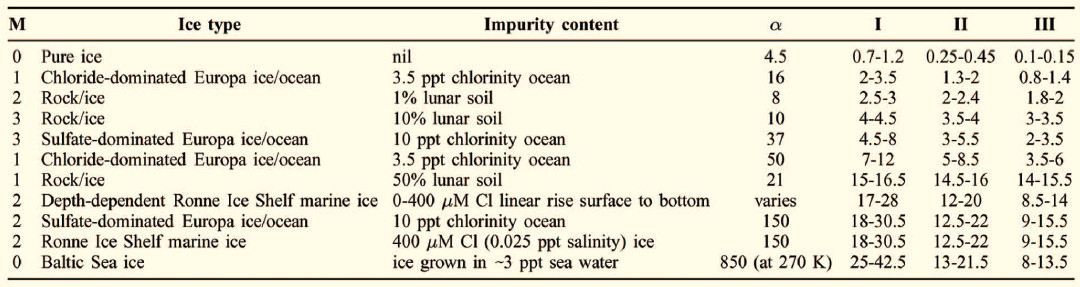
\includegraphics[width=1\textwidth]{figures/Moore2.jpg}
\caption{Attenuation, $a$, is in dB/km at 251 K and corresponds to the one way attenuation due to  ice impurities, in case of a sounding radar. Columns I, II, and III are computed one-way attenuation, in dB/km, for ice shells with base temperatures of 270, 260, and 250 K, respectively. The range of values for each of these corresponds to surface temperatures of 50 and 100 K. These values are independent of shell thickness since the temperature profile is stretched to the ice thickness. The M column represents the plausibility of the ice type for Europa; 0 is least likely while 3 is more likely, given the present understanding
of Europa. The distribution coefficients $k_{0}$ and $k_{MI}$ affecting the marine ice models come from laboratory experiments \cite{Moore_2000}. \textbf{+ appendix}}
\label{fig:impurities}
\end{figure}
The above calculations data are not taking into account a possible scattering mechanism of electromagnetic wave due to ice layers that can exist in the crust. The scattering effect has a significant impact on the attenuation level and depends strongly on the dimensions of cavities in the medium compared to the wavelength. The two main mechanisms of scattering coming from the ice crust are surface scattering and scattering by volume irregularities. Both these effects can change considerably the penetration depth of the wave into the ice, but also the ratio of any subsurface echo to surface clutter. As we can understand the scattering depends strongly on the wavelength and surface parameters of the body under investigation. 

The conclusion is that the expected one way attenuation because of impurities of ice is in the range 1-8 dB/Km and this number is independent of the frequency. Although, the frequency dependence of attenuation due to scattering mechanisms dictates the use of as low frequencies as possible in order to achieve a deep penetration. The main bottlenecks in that case are two. The first one is that the choice of frequency has an influence on the characteristics of instrumentation and especially on the size of the antenna and the second one is Jupiter's radio emissions spectrum. Figure \ref{fig:J_spec} depicts how Jupiter's activity affect the electromagnetic environment of its moons. Clearly can be seen that frequencies from almost zero Hz up to 50 MHz are dominated from Jupiter's radio emissions. Thus, the exact choice of frequency results in a trade off between science requirements and technical limitations taking into account also the physical constraints of the environment under research. 

\begin{figure}[htb]
\centering
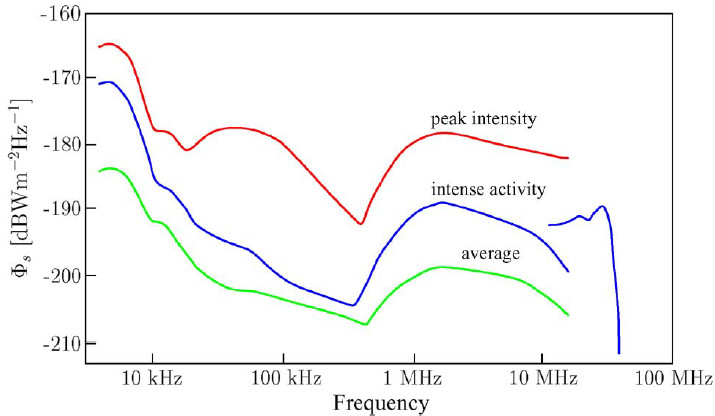
\includegraphics[width=0.7\textwidth]{figures/below100.jpg}
\caption{Jupiter radio spectrum based on Cassini-RPWS data,
normalized to a distance of 1 AU. Green curve: rotation averaged
emission. Blue curve: rotation averaged emission at times of intense
activity. Red curve: peak intensities during active periods. \cite{Grie_meier_2005}}
\label{fig:J_spec}
\end{figure}


\begin{figure}[htb]
\begin{center}
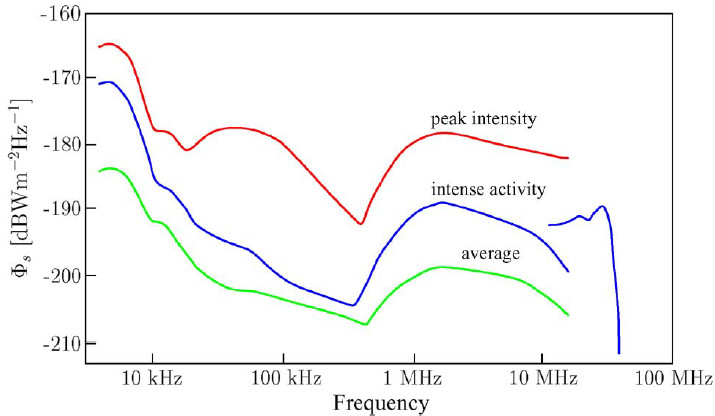
\includegraphics[width=0.7\columnwidth]{figures/below100}
\caption{Replace this text with your caption%
}
\end{center}
\end{figure}

\subsection{Communication to Lander}

\subsection{High Directivity Link}

\subsection{Relay Systems}
